%===============================================================================
% Template Name:      SUnORE Starter Presentation template
% Template URI:       http://sunore.co.za/sunore-presentation/
% Description:        Starter Presentation template for SUnORE 
%                     Department of Industrial Engineering, 
%                     Stellenbosch University
% Version:            1.1.0
% Author:             Johan Janse van Rensburg
% Author URI:         http://johanjvrens.co.za/
% License:            MIT License
% License URI:        http://opensource.org/licenses/MIT
%===============================================================================
\documentclass[serif,11pt]{beamer}

%=================================================
% theme and color
%=================================================
\usetheme{Warsaw} %Themes http://www.hartwork.org/beamer-theme-matrix/
\definecolor{colorA}{RGB}{96, 34, 59}
\definecolor{colorB}{RGB}{140, 151, 154}
%\definecolor{secinhead}{RGB}{249,196,95}
%\definecolor{titlebg}{RGB}{51,51,51}
\setbeamercolor{structure}{fg=colorA,bg=colorB}
%\setbeamercolor{secsubsec}{fg=secinhead,bg=black}
%\setbeamercolor{frametitle}{fg=secinhead,bg=titlebg}

%=================================================
% packages and new commands
%=================================================
\usepackage{colortbl}
%\usepackage[ruled, linesnumbered, vlined]{algorithm2e}
\usepackage{epsfig, subfigure, amssymb, multirow, algorithmic, amsmath}
\newcommand*{\superscript}[1]{\ensuremath{^{\rm #1}}}
\newcommand*{\subscript}[1]{\ensuremath{_{\rm #1}}}
\DeclareMathOperator*{\argmax}{arg\,max}

%=================================================
% thesis details (preamble)
%=================================================
\title[{\sc Optimizations of the Skip-Gram model with negative sampling} \hspace{0.8cm} \insertframenumber/\inserttotalframenumber]{{\sc Optimizations of the Skip-Gram model with negative sampling}}
\author[Optimizations Skip-Gram model--- {\sc Apr. 1\superscript{st}, 2019}]{{Milinaire Cédric}}
\date{1 April 2019}
\institute{Chair of Data Science \\  University of Passau, Germany}

%=================================================
% start presentation
%=================================================
\begin{document}

%========================
% title page
%========================
\begin{frame}
  \begin{center}
    \vspace{0.1cm}
    
\includegraphics[scale=0.3]{uplogo.png}
  \end{center}
  \titlepage
\end{frame}

%========================
% your slides:
%========================
 \begin{frame}
 \frametitle{Overview} 
 \begin{Large}
Overview of my thesis
 \end{Large}
 \bigskip
 \begin{itemize}
 \item Word embeddings are vector representations of words
 \item Word embeddings are a powerful tool that facilitate NLP
 \item Skip Gram Model with negative sampling, is a simple and powerful algorithm (Mikolov et al.) \cite{mikolov}
 \item This work focused on optimizing the convergence time
 \item Techniques used: 
 \begin{itemize}
 \item Advanced optimizers
 \item Input shuffling
 \end{itemize}
 \end{itemize}
 \end{frame}
\iffalse
\begin{frame}\frametitle{Motivation}
\textbf{How can we encode vectors for machine learning? }\\
\bigskip 
\centerline{
He =$
\left(
\begin{array}{c}
\rowcolor{green! 20}
1\\
0\\
0\\
\end{array}\right)
$
is = $
\left(
\begin{array}{c}
0\\
\rowcolor{blue! 20}
1\\
0\\
\end{array}\right)
$
King =
$
\left(
\begin{array}{c}
0\\
0\\
\rowcolor{red! 20}
1\\
\end{array}\right)
$}
\bigskip
\begin{itemize}
    \item \texttt{PROBLEMS:}
    \begin{itemize}
    \item All vectors have the same distance to each other
    \item Very high dimension 
    \end{itemize}
\end{itemize}
\end{frame}
\begin{frame}\frametitle {Motivation}
    \framesubtitle{Why are word embeddings necessary?}
    \textbf{We need a new system to create word embeddings }
      \begin{itemize}
 \item $\Rightarrow $Skip-Gram Model  (Mikolov et al. 2013) \cite{mikolov}
 \item Low dimension
 \item Captures meaning
 \item Speeds up and improves other NLP tasks, for example machine translation. 
 \end{itemize}
  \end{frame}
  \fi


\begin{frame}\frametitle{Outline}
\begin{enumerate}
\item Overview of my Thesis
\item Background
\begin{enumerate}
\item Skip Gram Model
\item Skip Gram Model with negative Sampling
\end{enumerate}
\item Implementation
\item Results
\item Discussion
\item Continuation of the Thesis
\item Conclusion
\end{enumerate}
	
\end{frame}
\begin{frame}\frametitle{Background}
\begin{Large}
Background
\end{Large}
\begin{enumerate}
\item Skip Gram Model 
\item Skip Gram with Negative Sampling (SGNS)
\end{enumerate}
\end{frame}
\begin{frame}\frametitle{Background}
Main idea: train a network on a "fake task" then use the weights as embedding. \bigskip
\begin{itemize}
\item The fake task:
\item Given a word $w$ guess the context words. 
%\item We want to maximize the following probability:
\end{itemize}
%\begin{equation}
%\prod_{t=1}^T \prod_{-m<j<m}  p(w_{t+j}|w_t)
%\end{equation}
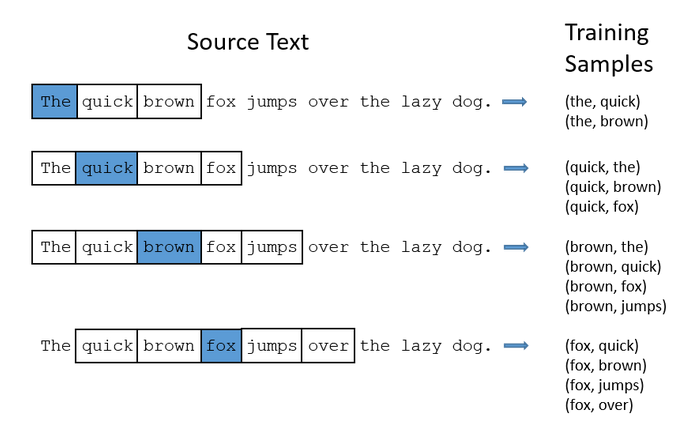
\includegraphics[scale=0.37]{images/context_pairs.png}
\end{frame}

\begin{frame}\frametitle{Background}\framesubtitle{Network achitecture}
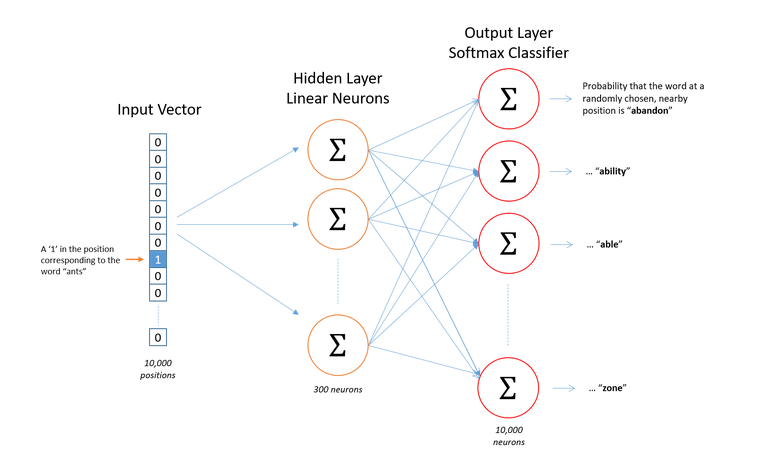
\includegraphics[scale=0.37]{images/ntw_architecture.png}
(Source: http://mccormickml.com/2016/04/19/word2vec-tutorial-the-skip-gram-model/) 
\end{frame}
\iffalse
\begin{frame}\frametitle{Background}\framesubtitle{Example}
$
\newcolumntype{g}{>{\columncolor{green! 20}}c}
\newcolumntype{b}{>{\columncolor{blue! 20}}c}
\newcolumntype{r}{>{\columncolor{red! 20}}c}
\left(
\begin{array}{cbc}
0 & 1 & 0 
\end{array}\right)
\left(
\begin{array}{ccc}
\rowcolor{green! 20}
1 & 1 & 1  \\
\rowcolor{blue! 20}
2 & 2 & 2 \\
\rowcolor{red! 20}
3 & 3 & 3 \\
\end{array}\right)
= 
\left(
\begin{array}{ccc}
\rowcolor{blue! 20}
2& 2 & 2
\end{array}\right)
\newcolumntype{g}{>{\columncolor{green! 20}}c}
\newcolumntype{b}{>{\columncolor{blue! 20}}c}
\newcolumntype{r}{>{\columncolor{red! 20}}c}
\left(
\begin{array}{gbr}
0.1 & 0.2&0.3  \\
0.1 & 0.2&0.3  \\
0.1 & 0.2&0.3 \\
\end{array}\right)
$
$
= 
\newcolumntype{g}{>{\columncolor{green! 20}}c}
\newcolumntype{b}{>{\columncolor{blue! 20}}c}
\newcolumntype{r}{>{\columncolor{red! 20}}c}
\left(
\begin{array}{gbr}
0.6 & 1.5 & 3 
\end{array}\right)
\implies Softmax:
\left(
\begin{array}{gbr}
0.13 & 0.31 & 0.56 
\end{array}\right)
$
$
c
$
\vspace{10pt}

$
p(v_{he}| v_{is})   
 $
 
 \vspace{10pt}
 
 $
 p(v_{king}| v_{is})
 $

\end{frame}
\fi

\begin{frame}\frametitle{Background}
   \begin{flalign}
\text{Softmax: } &&  p(c|w) =  \frac{exp( {v^{'}_c}^\intercal v_w )}{\sum_{i=1}^T exp({v^{'}_i}^\intercal v_{w})}
   \end{flalign}
  \hfill   $v^{'} $is the output layer vector
  $v$ is the input layer vector
\begin{large}
Negative Sampling
\end{large}
\begin{itemize}
\item Distinguish data from noise $\Rightarrow$ reduce problem to a logistic regression. 
\item Guess k random samples 
\item For each pair $(w,c)$ we get:
\medskip
\end{itemize}
  \begin{flalign}
 && \argmax_{\theta }\ log(\sigma({v^{'}_c}^\intercal v_w ) + \sum_{k\in K} log(\sigma(-{v^{'}_k}^\intercal  v_w ))  
  \end{flalign}
  \begin{itemize}
  \item Uses SGD as an optimizer
  \end{itemize}
\end{frame}

\begin{frame}
\frametitle{Background}
\begin{Large}
State of the Art
\end{Large}
\begin{itemize}
\item word2vec (Mikolov et al. 2013)  \cite{mikolov}
\item Parallelizing Word2Vec in Shared and Distributed Memory (Ji et al. 2016)\cite{intel}
\item Acceleration of Word2vec Using GPUs (Seulki and Youngmin  2016) \cite{gpu}
\item Gensim ({\v R}eh{\r u}{\v r}ek and Sojka) \cite{gensim}
\end{itemize}
\begin{Large}
Research Questions:
\end{Large}
\medskip \\
 Can the convergence time of the skip Gram Model be optimized by the use of:
\begin{itemize}
\item Advanced optimizers
\end{itemize}
and
\begin{itemize}
\item Input Shuffling
\end{itemize}
while at the same time maintaining it's accuracy? 
\end{frame}

\begin{frame}
\frametitle{Background}
\begin{Large}
Our Implementation \\
\end{Large}
Main Idea: 
\begin{itemize}
\item Create a large batch of training samples, i.e 2000 pairs
\item Compute loss for each pair
\item Use sum over all pairs as loss for batch 
\end{itemize}
\end{frame}
\begin{frame}
\frametitle{Background}
\begin{Large}
Our Implementation \\
\end{Large}
Illustration of the batched Skip-Gram Model
\\ $X = {(v_1,c_1),(v_2,c_2),(v_3,c_3)}$
Input:\\
 $v = \begin{bmatrix}
v_1 & v_2 & v_3
\end{bmatrix}, c = \begin{bmatrix}
c1\\
c2\\
c3\end{bmatrix}$ and $A = 
\begin{bmatrix}
k_{1,1} & k_{2,1} & k_{3,1}\\
k_{1,2} & k_{2,2} & k_{3,2}\\
k_{1,3} & k_{2,3} & k_{3,3}\\
\end{bmatrix}$\\

 We then concatenate $c$ and $A$, 
resulting in: \\
$\tilde{A} = \begin{bmatrix}
c_1 & k_{1,1} & k_{2,1} & k_{3,1}\\
c_2 & k_{1,2} & k_{2,2} & k_{3,2}\\
c_3 & k_{1,3} & k_{2,3}& k_{3,3}\\
\end{bmatrix}$

\end{frame}


\begin{frame}
\frametitle{Background}
\begin{Large}
Our Implementation \\
\end{Large}
Embeddings:\\
$E_v = \begin{bmatrix}
\tilde{v_1}_1 & \ldots & \tilde{v_1}_d\\
\tilde{v_2}_1 & \ldots & \tilde{v_2}_d\\
\tilde{v_3}_1 & \ldots & \tilde{v_3}_d\\
\end{bmatrix}
$, where $\tilde{v_i} = \begin{bmatrix}
\tilde{v_i}_1 & \ldots & \tilde{v_i}_d \end{bmatrix}$ is the embedding of $v_i$.  \\$E_c = \begin{bmatrix}
\tilde{c_1 }& \tilde{k_{1,1}} & \tilde{k_{2,1}} \\
\tilde{c_2 }& \tilde{k_{1,2}}& \tilde{k_{2,2}} \\
\tilde{c_3 }&\tilde{ k_{1,3} }& \tilde{k_{2,3}}\\
\end{bmatrix}$,
where each entry of the matrix is a vector of dimension $d$\\

Batch multiplication and negation of samples:\\
$S = \begin{bmatrix}
\tilde{v_1} \cdot  \tilde{c_1} & -\tilde{v_1} \cdot \tilde{k_{1,1}} & -\tilde{v_1} \cdot  \tilde{k_{2,1}}& -\tilde{v_1} \cdot  \tilde{k_{3,1}}\\
\tilde{v_2} \cdot \tilde{c_2} & -\tilde{v_2} \cdot \tilde{k_{1,2}} & -\tilde{v_2} \cdot \tilde{k_{2,2}} & -\tilde{v_2} \cdot \tilde{k_{3,2}}\\
\tilde{v_3} \cdot \tilde{c_3} &-\tilde{v_3} \cdot c_3  \tilde{k_{1,3}} & -\tilde{v_3} \cdot c_3 \tilde{k_{2,3}}&-\tilde{v_3} \cdot \tilde{k_{3,3}}\\
\end{bmatrix}$\\

Loss computation: \\
 L = $- \sum_{(i,j) \in k \times n} S(i,j) $

\end{frame}

\begin{frame}\frametitle{Implementation}
\begin{Large}
Implementation
\end{Large}
\begin{enumerate}
\item Setting
\begin{itemize}
%\item Hardware Specs
\item Dataset 
\item Network Architecture 
\end{itemize}
\item Optimization Process
\end{enumerate}
\end{frame}
%%%%%%%% Specs not in pres
\iffalse
\begin{frame}
\frametitle{Hardware Specs} 
\begin{itemize}
\item Intel(R) Xeon(R) CPU E5- 2650 v3 @ 2.30GHz
\item CPU(s):                40
\end{itemize}
\end{frame}
\fi
\begin{frame}
\frametitle{Dataset} 
    \begin{itemize}
\item Text8 dataset
\item First 30MB of clean text from wikipedia 
\item Vocabulary $\approx$ 250k word (small) 
\item Subsampling $\implies$ 50\% decrease of data set size
\end{itemize}
\end{frame}

\begin{frame}
\frametitle{Optimization process}
Optimization techniques:
\begin{itemize}
\item Advanced Optimizers
\begin{itemize}
\item Momentum
\item Nesterov accellerated Momentum 
\item Adagrad 
\item Adam
\end{itemize}
\item Input Shuffling
\end{itemize}
\end{frame}



\section{Results}\label{sec:results}
We ran multiple experiments for each optimizer. This Section will  give an overview of the achieved results. Each subsection will give an explanation over the achieved result with a specific optimizer.

\subsubsection{SGD}
The first challenge for each optimizer was to find a correct learning rate. As SGD is the optimizer used in Gensim \cite{gensim} we first tried the same learning rate as the default value in Gensim \cite{gensim}, i.e 0.01,  and then performed a random search to find a better one. As expected a bell curve shape resulted, a learning rate that is too high leads to diversion and a learning rate that is too low leads to a training time that is too slow. The best value that we found for the learning rate is $0.0075$. With this setting SGD converged in 11 epochs. The second experiment was to add input shuffling.
As seen in Figure \ref{fig:results_sgd}, for almost every learning rate the convergence time decreased. Our model, with the best setting, now converges in only 7 epochs. Another interesting fact to point out from Figure \ref{fig:results_sgd} is that with input shuffling we achieved better results with higher learning rates. As for learning rates of $0.01$ and $0.025$ we did converge in 11 epochs with input shuffling but did not converge in 20 epochs without it.

\begin{figure}[h]
\centering
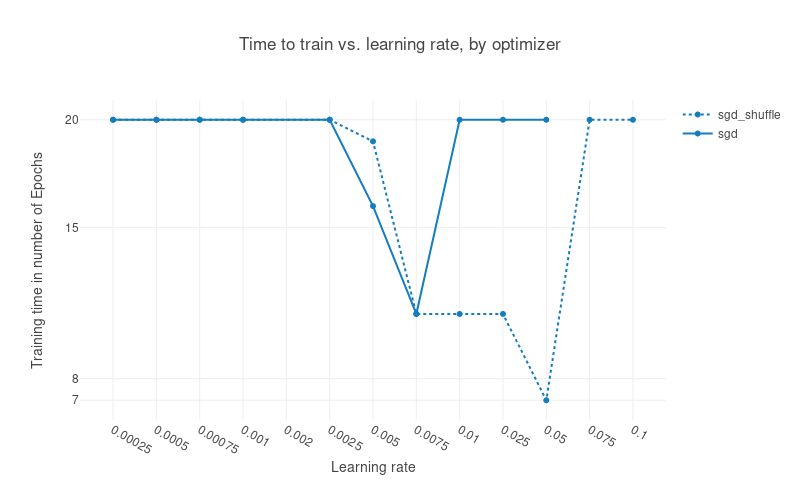
\includegraphics[scale=0.3]{images/results_sgd_shuffle}
\caption{Training time Stochastic Gradient Descent with input Shuffling}
\label{fig:results_sgd}
\end{figure}
\subsubsection{Momentum and Nesterov}
Momentum and NAG \cite{nag} both have an additional hyperparameter $\gamma$, that, defines the percentage of the previous gradient that will be added to the current gradients. We set $\gamma = 0.9$ as this is a typical value and did not alter it during our experiments. Momentum and Nesterov alone respectively only slightly decrease or increase the convergence time. Momentum optimally converges in 9 epochs and Nesterov in 13. If we combine these optimizers with input shuffling, interestingly the same phenomena as with plain SGD appear. The convergence time gets better, 8 epochs for Momentum and 3 epochs for NAG. The phenomena that a higher learning rat yields better results also happens with both of the optimizers. As Momentum does not converge in 20 epochs with a learning rate of 0.002 but does in 8 with input shuffling.
\begin{figure}[h]
\centering

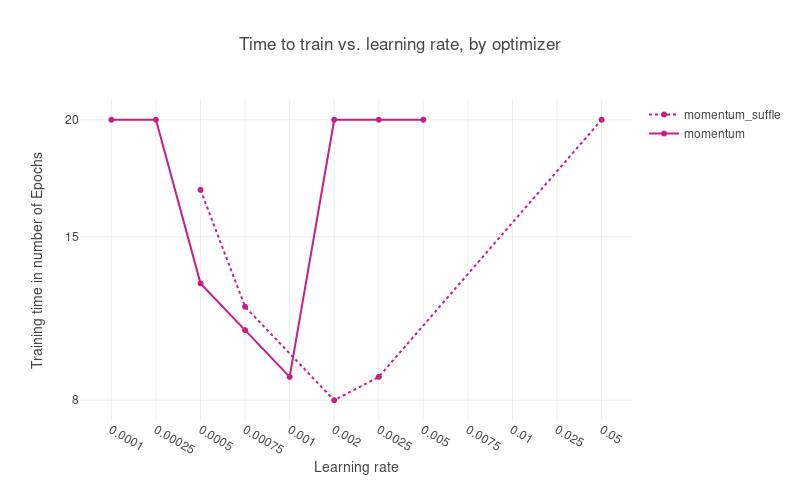
\includegraphics[scale=0.3]{images/results_mom_shuffle}
\caption{Training time Momentum with input Shuffling}
\label{fig:results_mom}
\end{figure}

\begin{figure}[h]
\centering
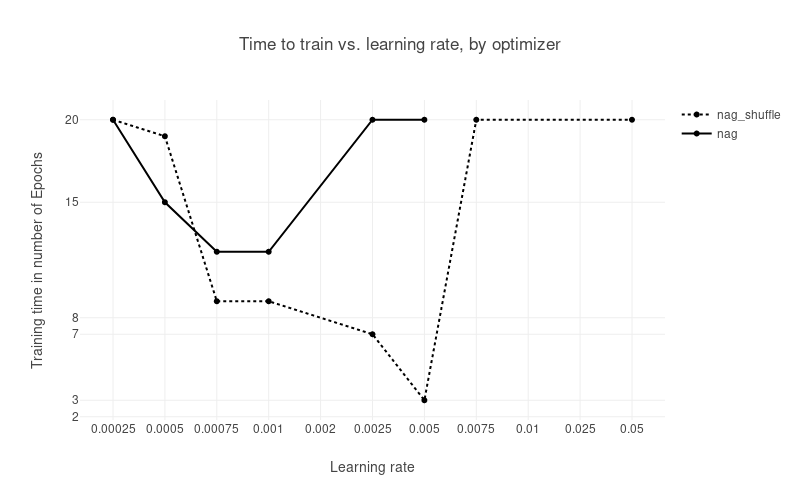
\includegraphics[scale=0.3]{images/results_nag_shuffle}
\caption{Training time Nesterov with input Shuffling}
\label{fig:results_nag}
\end{figure}
\subsubsection{Adagrad}
Adagrad \cite{adagrad} is a very interesting tool for learning word embeddings as it decreases the learning rate for very frequent occurring features, and vice versa). Because words that appear very frequently often do not have a semantic gain that is as important as words that appear less frequently to their context words, it's good to have a lower learning rate for such frequent words. So, in theory, Adagrad is particularly well suited for our task, as for example Pennington et al. used Adagrad in the training of Glove \cite{glove}, another system used to create word embeddings.  This was confirmed empirically as our model converged in 4 epochs. When combined with shuffling Adagrad only took 3 epochs to converge. This shows the tendency of the skip gram model to converge faster with input shuffling and the big impact of having different learning rate for each feature.
Here it's interesting to notice that a higher learning rate combined with input shuffling did not yield better results than without shuffling. Both of our best results happened with a learning rate of $0.1$, as shown in Figure \ref{fig:results_adagrad_shuffle}.
\begin{figure}[h]
\centering
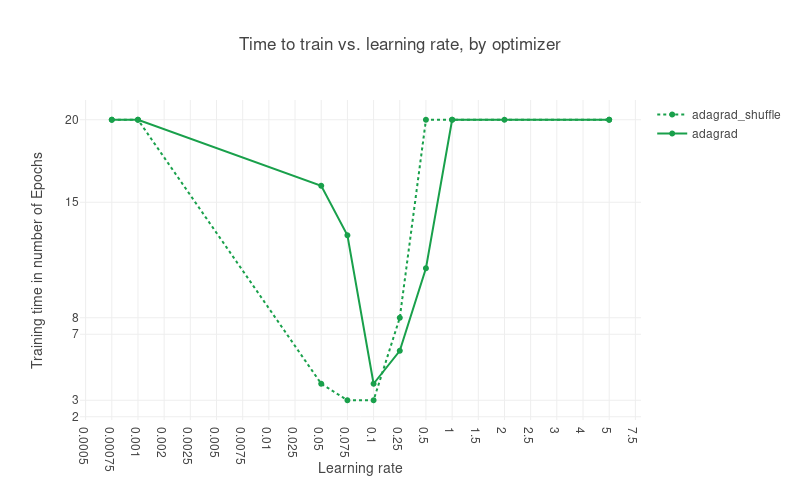
\includegraphics[scale=0.3]{images/results_adagrad_shuffle}
\caption{Training time Adagrad with input Shuffling}
\label{fig:results_adagrad_shuffle}
\end{figure}
\subsubsection{Adadelta}
In theory Adadelta \cite{adadelta} should outperform Adagrad as it's an extension of the former. Because it didn't have any learning rate to tune, we only did 2 experiments, with and without input shuffling. 
We are aware of the fact that there are additional hyper parameters to Adadelta. We decide not to tune theim for to reasons: first for simplicity reasons and second because their effect is not as high as the learning rate. The parameter that defines the percentage taken when calculating the exponentially decaying average of past gradients was set to $\rho = 0.9$. Adadelta did not manage to achieve a word similarity of 0.66. It only converged to a similarity of 0.59. It did this in 20 epochs without input shuffling and in 3 with input shuffling, as can be seen in Table \ref{table:results_adadelta}


\begin{table}[tb]
    \caption{Convergence Time and Quality with Adadelta}
    %\scriptsize
    \begin{tabular}{l r r }%
        \toprule
Adadelta Model & Convergence Time & Word similarity \\ 
        \midrule%
        Without Shuffling & 20 & 0.59 \\ 
With Shuffling & 3 & 0.59 \\
        \midrule%
   \end{tabular}%
   \label{table:results_adadelta}%
\end{table}

\subsubsection{Adam}
Adam is the most advanced of all the optimizers used in our experiments and did yield the best results as seen in Figure \ref{fig:results_adam_shuffle}. Adam converged in 3 epochs without shuffling and 2 with. This is the best result that we got with any optimizer.  It's also interesting to note that as same as with Adagrad it did not react to input shuffling the same way as SGD did. In fact, it worked in the opposite direction, as we achieved our best result with input shuffling while having a lower learning rate $0.001$ then we used to achieve the best result without input shuffling $0.05$.
\begin{figure}[h]
    \centering
            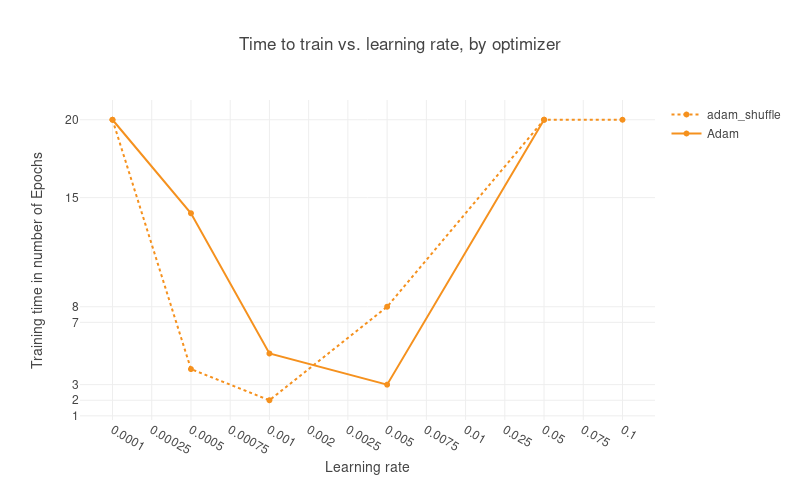
\includegraphics[scale=0.3]{images/results_adam_shuffle} 
    \caption{Training time Adam with input Shuffling}
    \label{fig:results_adam_shuffle}
\end{figure}
\section{Discussion}\label{sec:discussion}

%Discuss the results. What is the outcome of your experimetns?
This section shortly discusses the empirical results and then extensively compares the findings of this work to the existing literature while trying to explain some of the differences. It is concluded by a subsection describing the limitations and possible extensions of this work. 

\subsection{Our work}
This subsection discusses our findings. First it will analyze the possible reasons behind the influence of input shuffling to the learning rate. Second it will conclude with the discussion of unexpected results. 

\subsubsection{Shuffling and learning rate with SGD}
In this subsubsection we will use the term SGD for SGD, Momentum and NAG, and advanced optimzers for Adagrad and Adam. The models was able to use a higher learning rates when SGD optimizers where combined with input shuffling in comparison to as when not, as shown in Figures \ref{fig:results_sgd}, \ref{fig:results_mom} and \ref{fig:results_nag}. Therefore, arises the questions why these phenomena happen, especially as it did not happen with advanced optimizers.  \\
First, we suspect our batched version of the Skip-Gram model with negative sampling (SGNS), to be at the origin of this phenomena. In consequence to this batched version, when input shuffling is not used a lot of words will appear multiple times in the same batch, as explained in Section \ref{ssec:shuffling}. Therefore, the gradients will be an average of all the training samples. When the input is shuffled, less words will appear multiple time which will make the gradients more precise.\\
Second, advanced optimizers have a way to counter-attack this issue, namely adaptive learning rates, explained in Section \ref{ssec:results_adagrad}. Adaptive learning rates counter attack the issue in the following way: high frequency words  will appear more often multiple times in a batch, they will also have lower learning rates. Therefore the impact of appearing in the same batch will be reduced. \\  The two above arguments could explain why a higher learning rate combined with SGD achieved better results with input shuffling but not when advanced optimizers are used. 

\subsubsection{Large differences with NAG and SGD when using shuffling}
SGD and NAG both have very different values when using shuffling in comparison to unshuffled input, as shown in figures \ref{fig:results_sgd} and \ref{fig:results_nag}. We do not only attribute those results to input shuffling but partially also to a good random initialization guess. Due to a lack of time these experiments were not replicate more than once.

\subsection{Comparison to Gensim}
This subsection will compare our finding extensively to Gensim \citep{gensim}. As explained in Section \ref{ssec:gensim}, Gensim is optimized to have a very high throughput, this made it possible to achieve a lot of computations. Furthermore, Gensim provides access to the loss and the resulting word embeddings, which facilitated the comparison process.
This subsection is structured as follows: first it will describe the used configuration of Gensim, second it will compare Gensim to our implementation of the SGNS with the use of SGD and finally compare our model with Adam to Gensim. A graphic showing the comparison of our models to Gensim can be found in Figure \ref{fig:gensim_vs_adam}.


\subsubsection{Configuration of Gensim}
To compare our-self in a correct  manner we used the same dataset, with the same preprocessing parameters, i.e subsampling and min count. The hyper parameters of the network (window size, embedding size, number of negative sample, exponent to which the unigram distribution, which decides how a negative sample is used, is raised) are equivalent to our parameters described in Section \ref{ssec:config}. The only difference with our model is the learning rate. Gensim has a starting learning rate of $0.025$ and linearly decrease it at every epoch to $0.0001$.

\subsubsection{Gensim vs. SGD}
As stated earlier, we are not going to compare this work to Gensim in run time. Gensim is heavily optimized and written in cython\footnote{https://rare-technologies.com/word2vec-in-python-part-two-optimizing/}, which is 23x faster than plain Numpy. Since we used PyTorch the difference is not that big, but still remains. As shown in Figure \ref{fig:gensim_vs_adam} the convergence time was not the same between our implementation and Gensim. There are different possible reasons why this could be the case:\\ First, our batched approach could hinder performance in terms of convergence time since our loss function is not exactly the same. We compute the loss for multiple training samples by taking the sum over each score which is individually used as a loss by Gensim.\\ Secondly, a difference to our implementation is the fact that Gensim checks whether negative samples are not equal to the context word. If that is the case Gensim selects a new random sample. Therefore, the learning of the input and output context is optimized. \\Finally, another possibility is the decay of the learning rate used by Gensim. In fact, decaying the learning rate has been proven in a lot of work to decrease the convergence time. Gensim linearly decreases the learning rate, as we did not use this technique, the decay of the learning rate could help explain the noted differences. \\ The first hypothesis, the fact that we used a batched approach, may be confirmed by the fact that when combined with input shuffling SGD does perform closer to Gensim, going from 11 to 7 epochs to converge, as input shuffling reduces the number of co-occurrence of the same word in a batch.
Know the question arises if the 3 epochs, that Gensim is better, can be explained by the selection of better negative samples and the learning rate decay.

\subsubsection{Gensim vs. Adam}
The Adam optimizer did outperform the Gensim application in quality of word embeddings (only slightly: 0.01 correlation coefficient better) and convergence time. Adam converged in 2 epochs while Gensim in 4. To confirm the achieved results we ran each computation 40 times. The results can be seen in Figure \ref{fig:gensim_vs_adam}.

\begin{figure}[h]
\centering
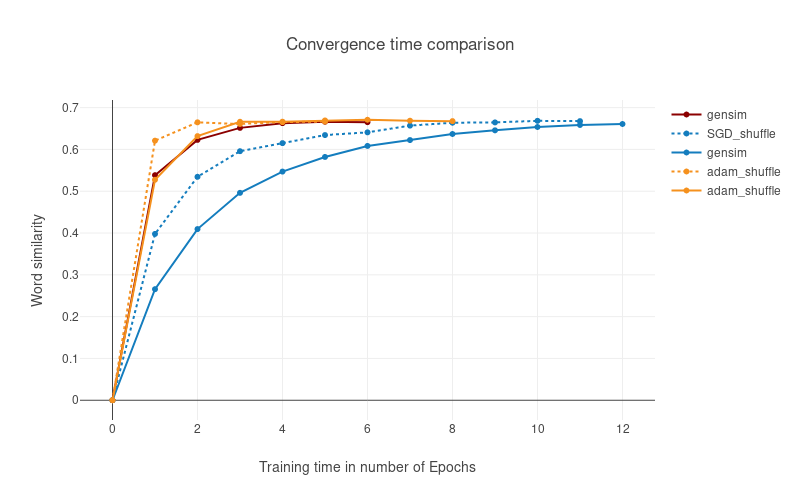
\includegraphics[scale=0.3]{images/gensim_vs_adam}
\caption{Convergence time of SGD and Adam compared to Gensim}
\label{fig:gensim_vs_adam}
\end{figure}

\subsection{Future Work}
This work shows that the convergence time of the SGNS could be improved by using input shuffling and advanced optimizers. As with every work, there still exists possible extensions. First and foremost an aspect of our implementation that can be prejudicial is that we only extensively tested our model with one small dataset. The fact that we only used one dataset as well that it's a small one is problematic. \\ 
~~\textit{Problem with a small dataset:} \\ By using a very small dataset we do not use the model in the condition it is most needed for, as the dataset used in practice usually consists of more than 1 billion words. There is a small argument that can be made for machine translation as the use of small parallel corpus is not unusual in this field. \\
~~\textit{Problem with using only one dataset:}\\
It has been shown that some optimizers perform better with specific shapes of loss functions. To make a compelling argument it's necessary to show that our model with the use of input shuffling and Adam as its optimizer also outperforms Gensim with other data sets.\\
Finally, as it wasn't the goal of our implementation to outperform Gensim in run time, one could improve an already existing, optimized version, with input shuffling and advanced optimizers and should achieve a better run time than Gensim.

\section{Conclusion}\label{sec:conclusion}

This work provides an overview of the Skip Gram Model with negative Sampling (SGNS) and the numerous successful attempts of optimizing the throughput of the model. As this is the case, no effort went into optimizng the convergence time of the SGNS, therefore this work focused on this point. We decided to use advanced optimizers and input shuffling as optimizing techniques. After giving a short overview over Gradient Descent algorithms this work proposes a slighlty altered version of the SGNS, where the idea is to compute the loss over the sum of a high number of training samples, i.e 2000,  instead of computing it for each individually.  We did this as it allowed us to compute more models and analyze the convergence time faster. We used the text8 dataset and used  word similarity as a quality measure for the word embeddings (WE). We used the State of the art implementation Gensim to compare our self. We did achieve a better convergence time than gensim with Adam as an optimizer and the use of input shuffling. Gensim convereged in 4 epochs to a word similarity of 0.66 and our model only took 2 epochs to achieve the same quality. Those results still need to be confirmed with more datasets. Finally, if this work would be combined with an optimized throughput it  could improve the state of the art run time of the SGNS.

  \begin{frame}
\frametitle{Delete double occurrences}
\begin{Large}
How can we improve the batched approach? \\
\end{Large}
\begin{Large}
Problem:\\
\end{Large}
Words appear more than once in a batch $\rightarrow$ performance loss\\
\begin{Large}
Solution:\\
\end{Large}
Create batch of different sizes, each batch will hold at most one pair per context word\\
  \end{frame}

  
    \begin{frame}
\frametitle{Delete double occurrences}
\begin{Large}
Sentence = The fox jumps over the dog\\
Example Dictionnary:\\
\end{Large}
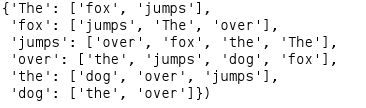
\includegraphics[scale=0.5]{images/dict_ex}\\
\begin{Large}
Example Batches
\end{Large}
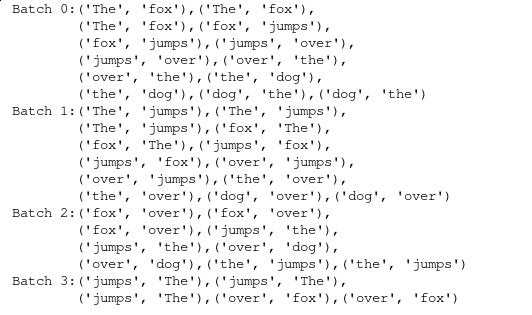
\includegraphics[scale=0.4]{images/batch_ex}
  \end{frame}
  
   \begin{frame}
\frametitle{Delete double occurrences}
\begin{large}
Problem of the Solution:\\
\end{large}
Average Batch Size = 200, i.e training takes too long
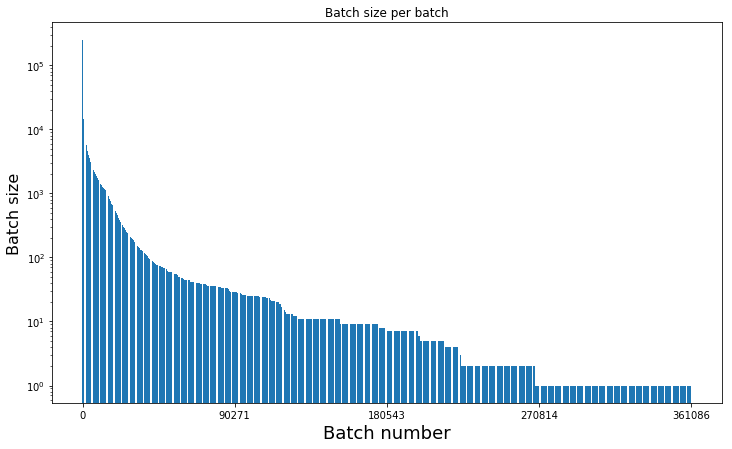
\includegraphics[scale=0.34]{images/batch_sizes}
  \end{frame}  
  
  
\begin{frame}
\frametitle{Distribution of Words}
\centering
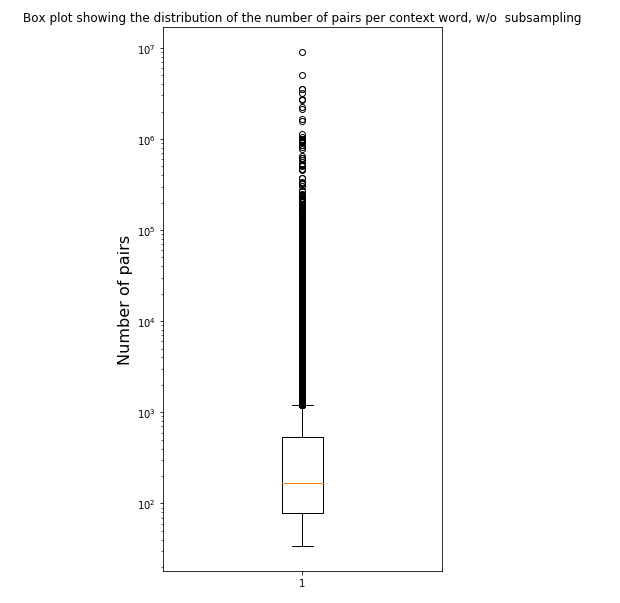
\includegraphics[scale=0.4]{images/no_sampling_boxplot}
  \end{frame}
\begin{frame}
\frametitle{Distribution of Words}
\begin{Large}
Results of the Distribution
\end{Large}
\begin{itemize}
\item A few words are responsible for the majority of pairs. 
\item They almost have the same context words
\item Idea: delete outliers from dataset
\end{itemize}
  \end{frame}

    \begin{frame}
\frametitle{Deletion of outliers}
\begin{Large}
First Results 
\end{Large}
    \begin{table}[]
\begin{tabular}{|l|l|l|}
\hline
Model    & Convergence Time & Word Similarity \\ \hline
SGD & {11}              & 0.65            \\ \hline
SGD w/shuffling & {7}              & 0.66            \\ \hline
Adam & {3}              & 0.66            \\ \hline
Adam w/ shuffling & {2}              & 0.66      \\ \hline
Gensim   & 4          & 0.66            \\ \hline
Adam w/o outliers  & \textbf{1} & 0.66 \\ \hline
\end{tabular}
\end{table}
  \end{frame}
  
  
      \begin{frame}
\frametitle{Deletion of outliers}
\begin{Large}
Future Work 
\end{Large}
\begin{itemize}
\item Creating the perfect batch 
\item Analyze the deletion of outliers on other (bigger) datasets.
\item Confirm all results on other task
\end{itemize}
  \end{frame}
\begin{frame}\frametitle{Background}\framesubtitle{Softmax}
\begin{Large}
It's unsuitable to compute the softmax
\end{Large}
   \begin{equation}
  p(c|w) =  \frac{exp( {v^{'}_c}^\intercal v_w )}{\sum_{i=1}^T exp({v^{'}_i}^\intercal v_{w})}
   \end{equation}
   \begin{itemize}
   \item $v_w$ and $v^{'}_c$ are the "input" and "output" representation of $w$
\item For each pair we have to go over the whole training corpus. (Billions of word in practice) 
   \end{itemize}
\end{frame}


\begin{frame}
\frametitle{Network Architecture} 
\begin{columns}
    \column{0.6\textwidth}
\begin{itemize}
\item Dimension of input and output vectors = 100
\item Context window  = 5
\end{itemize}
    \column{0.6\textwidth}
    \begin{itemize}
    \item Negative Samples = 10 
\item Coded in Pytorch 1.0
\end{itemize}
  \end{columns}
  \bigskip
\begin{columns}
    \column{0.4\textwidth}
    		First 10 pairs of training:
        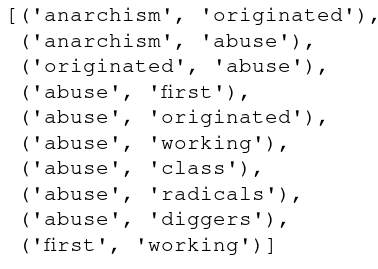
\includegraphics[scale=0.35]{images/pairs_example}    \column{0.6\textwidth}
        Negative Samples:\\
        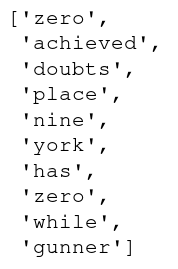
\includegraphics[scale=0.35]{images/neg_samples_example}
  \end{columns}
\end{frame}

\begin{frame}
Each parameter $\theta_i$, at time step $t$ will have it's own learning rate $\eta_{t,i}$
 \begin{equation}
\eta_{t,i} = \frac{\eta_0}{\sqrt{\sum^{t}_{i=1} g^{2}_{t,i}} \epsilon}
\end{equation}
where
\begin{itemize}
\item $g_{t,i} = \nabla J(\theta_{t,i})$  is the partial derivative of the loss function with respect to the parameter $\theta_i$ at time step $t$. 
\item each parameter $\theta_{i}$ has it's one learning rate
\item  $ \theta_{t+1,i} = \theta_{t_i} - \eta_{t,i} g_{t,i} $
\end{itemize}
We can now construct our global parameter update as follows: 
\begin{equation}
\theta_{t+1,i} = \theta_{t_i}- \frac{\eta}{\sqrt{G_{t_{i,i}}} + \epsilon} g_{t,i}, 
\end{equation} 
with  $G_{t_{i,i}}$ being the diagonal Matrix of the sum of the squares of the graditents ($g_{t,i} $).
\end{frame}

\begin{frame}\frametitle{Background}\framesubtitle{Softmax}
\centerline{
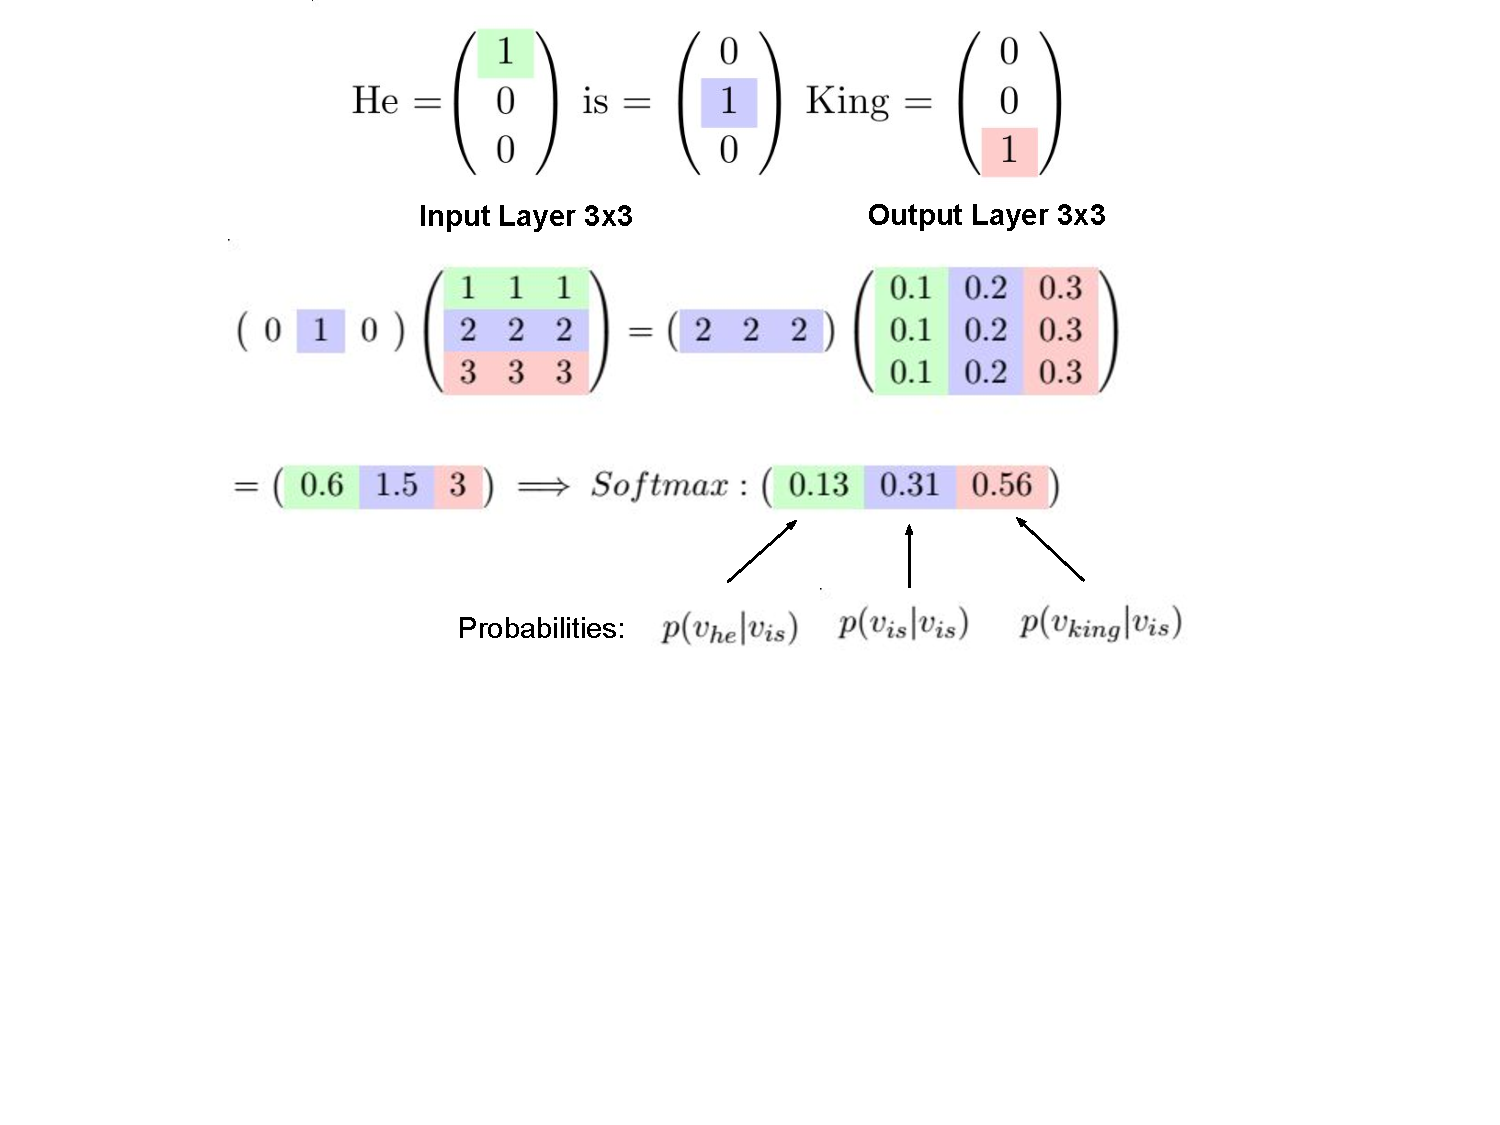
\includegraphics[scale=0.5]{images/skip_gram_example.pdf}}
\end{frame}
%========================
% example slides:
%========================

%========================
% bibliography
%========================
%%%%%%%%%%%%%%%%%%
%
% bibliography
%
%%%%%%%%%%%%%%%%%%

\begin{frame} \frametitle{References}
\begin{thebibliography}{xx}\footnotesize

\bibitem{mikolov} {\sc Mikolov, Tomas and Sutskever, Ilya and Chen, Kai and Corrado, Greg S and Dean, Jeff}, 2013, {\em Distributed representations of words and phrases and their compositionality }

\bibitem{intel} {\sc Ji, Shihao and Satish, Nadathur and Li, Sheng and Dubey, Pradeep}, 2016, {\em Parallelizing word2vec in shared and distributed memory}

\bibitem{gpu} {\sc Bae, Seulki
and Yi, Youngmin}, 2016, {\em Acceleration of Word2vec Using GPUs}

\bibitem{gensim} {\sc Radim {\v R}eh{\r u}{\v r}ek and Petr Sojka}, 2010, {\em Software Framework for Topic Modelling with Large Corpora}




\end{thebibliography}
\end{frame}

%=================================================
% end presentation
%=================================================
\end{document}
